\begin{document}
\section{Esempi di generazione di test}

In questo capitolo descriviamo 12 test set per JSetL, mostrando per ciascuno di essi il file di input \texttt{testX\_prolog\_data.txt}, e laddove significativo, anche parti dei file \texttt{testX\_java\_data.txt} e dei file Java finali.\\

Oltre all'intento ovvio di testare in generale i vincoli di JSetL, lo scopo di questi test set è anche quello di fornire una dimostrazione pratica di come affrontare alcuni scenari frequenti in cui l'utente potrebbe ritrovarsi (es.: testare vincoli definiti da utente, vincoli i cui argomenti condividono più variabili, vincoli su insiemi RIS (Restricted Intensional Set), vincoli su relazioni, ...).\\

\subsection{test1: eq, disj, union - casi standard}
Questo test set testa tre vincoli basilari di \texttt{LSet} in casi standard, ossia senza variabili ripetute negli insiemi.\\
\begin{itemize}
\item Constraint \textbf{eq}(LSet s): soddisfacibile $\iff$ \texttt{this} $=$ \texttt{s} (ovvero se l'\texttt{LSet} \texttt{this} unifica con l'\texttt{LSet} \texttt{s}).
\item Constraint \textbf{disj}(LSet s): soddisfacibile $\iff$ \texttt{this} $\cap$ \texttt{s} $=$ $\varnothing$.
\item Constraint \textbf{union}(LSet s, LSet q)}: soddisfacibile $\iff$ \texttt{q} $=$ \texttt{this} $\cup$ \texttt{s}.
\end{itemize}

\clearpage

Vengono di seguito riportati i file di specifica Prolog e Java, e una parte del file \texttt{EqTest.java}.\\

\texttt{test1\_prolog\_data.txt}
\lstinputlisting{code/test1/test1_prolog_data.txt}

\vspace{10 mm}

\texttt{test1\_java\_data.txt}
\lstinputlisting{code/test1/test1_java_data.txt}

\vspace{10 mm}

\texttt{EqTest.java}
\begin{lstlisting}
public class EqTest {
	
	@Test
	public void testEq_Aperto_Aperto() {
		Solver solver = new Solver();
		LSet A1 = new LSet("B1").ins(new LVar("A1"));
		LSet A2 = new LSet("B2").ins(new LVar("A2"));
		solver.add(A1.eq(A2));
		assertTrue(solver.check());
	}

	@Test
	public void testEq_Aperto_Chiuso() {
		Solver solver = new Solver();
		LSet A1 = new LSet("B1").ins(new LVar("A1"));
		LSet C2 = LSet.empty().ins(new LVar("X2")).ins(new LVar("Y2"));
		solver.add(A1.eq(C2));
		assertTrue(solver.check());
	}

	@Test
	public void testEq_Aperto_Var() {
		Solver solver = new Solver();
		LSet A1 = new LSet("B1").ins(new LVar("A1"));
		LSet V2 = new LSet("S2");
		solver.add(A1.eq(V2));
		assertTrue(solver.check());
	}

	@Test
	public void testEq_Aperto_Vuoto() {
		Solver solver = new Solver();
		LSet A1 = new LSet("B1").ins(new LVar("A1"));
		LSet E2 = LSet.empty();
		solver.add(A1.eq(E2));
		assertFalse(solver.check());
	}
	
	// altri 12 metodi di test

}
\end{lstlisting}

\subsection{test2: in, nin}
Questo test set testa i seguenti due vincoli di \texttt{LSet}:\\
\begin{itemize}
\item Constraint \textbf{in}(LSet s): soddisfacibile $\iff$ \texttt{this} $\in$ \texttt{s}.
\item Constraint \textbf{nin}(LSet s): soddisfacibile $\iff$ \texttt{this} $\notin$ \texttt{s}.
\end{itemize}

In particolare, si è stabilito che \texttt{this} fosse sempre una \texttt{LVar} come espediente per mostrare l'uso della sintassi \texttt{***}: come visto nel capitolo 4.1.3 infatti, inserendo questa stringa speciale in posizione i-esima tra i valori di un argomento, l'effetto ottenuto è quello che il vincolo non avrà mai quell'argomento in posizione i-esima.\\
Grazie a questa sintassi (utile anche in test successivi, come in test3 e test9) è possibile ad esempio decidere che in prima posizione dovranno apparire solamente \texttt{LVar}.\\\\

Viene di seguito riportato il file di specifica Prolog.\\

\texttt{test2\_prolog\_data.txt}
\lstinputlisting{code/test2/test2_prolog_data.txt}

%\texttt{test3\_java\_data.txt}
%\lstinputlisting{code/test3/test3_java_data.txt}

\subsection{test3: eq, disj, union - casi speciali}
Questo test set testa gli stessi vincoli del test1, ma in casi speciali.\\
In particolare, si sono scelte due categorie di casi speciali: insiemi in cui compare una stessa variabile ripetuta più volte e variabili esterne che compaiono in insiemi diversi.\\
Il primo caso speciale è utile per verificare che i duplicati vengano effettivamente eliminati in un \texttt{LSet}, mentre il secondo caso speciale è utile per verificare la falsità del paradosso di Russell.\\
Queste due casistiche sono ottenute ancora una volta grazie alla sintassi \texttt{***}, come visibile nei file di specifica Prolog e Java (in quello Java, si noti l'utilizzo della sezione \texttt{\$\$\$ local \$\$\$}).\\\\\\

\texttt{test3\_prolog\_data.txt}
\lstinputlisting{code/test3/test3_prolog_data.txt}

\vspace{10 mm}

\texttt{test3\_java\_data.txt}
\lstinputlisting{code/test3/test3_java_data.txt}

\vspace{10 mm}

I due casi speciali sopra menzionati sono testati in particolare dai seguenti due metodi generati:\\

\begin{lstlisting}
	//Eliminazione dei duplicati
	@Test
	public void testEq_Chiuso_Chiuso() {
		LSet A = new LSet("A");
		LSet B = new LSet("B");
		
		Solver solver = new Solver();
		LSet C1 = LSet.empty().ins(A);
		LSet C2 = LSet.empty().ins(A).ins(A);
		solver.add(C1.eq(C2));
		assertTrue(solver.check());
	}
	
	//... altri metodi di test...
	
	//Paradosso di Russell
	@Test
	public void testEq_Var_Aperto2() {
		LSet A = new LSet("A");
		LSet B = new LSet("B");
		
		Solver solver = new Solver();
		LSet V1 = A;
		LSet A1 = new LSet("R").ins(A);
		solver.add(V1.eq(A1));
		assertFalse(solver.check());
	}
\end{lstlisting}

\end{itemize}

\clearpage

\subsection{test4: vincolo utente}
Questo test set ha lo scopo di mostrare come testare un vincolo definito da utente.\\
Si è scelto di testare il seguente vincolo:

\begin{itemize}
\item Constraint \textbf{myTest}(LSet A, LSet B, LSet C): \\
soddisfacibile $\iff$ \texttt{A} $\cup$ \texttt{B} $=$ \texttt{C} $\wedge$ \texttt{A} $\cup$ \texttt{B} $\neq$ \texttt{C}.\\
(il vincolo è volutamente sempre falso).\\
\end{itemize}

Vengono di seguito riportati i file di specifica Prolog e parte di quello Java (in particolare, la sezione \texttt{\$\$\$ global \$\$\$}).\\

\texttt{test4\_prolog\_data.txt}
\lstinputlisting{code/test4/test4_prolog_data.txt}

\vspace{10 mm}

\texttt{test4\_java\_data.txt}
\lstinputlisting[firstline=1,lastline=4]{code/test4/test4_java_data.txt}

\subsection{test5: diff, inters, subset}
Questo test set ha lo scopo di testare tre ulteriori vincoli di \texttt{LSet} aventi la caratteristica di essere vincoli composti: sono ottenuti come congiunzione di altri vincoli.\\

\begin{itemize}
\item Constraint \textbf{diff}(LSet s, LSet q): soddisfacibile $\iff$ \texttt{q} $=$ \texttt{this} $\setminus$ \texttt{s}.
\item Constraint \textbf{inters}(LSet s, LSet q): soddisfacibile $\iff$ \texttt{q} $=$ \texttt{this} $\cap$ \texttt{s}.
\item Constraint \textbf{subset}(LSet s): soddisfacibile $\iff$ \texttt{this} $\subseteq$ \texttt{s}.
\end{itemize}

Viene di seguito riportato il file di specifica Prolog.\\

\texttt{test5\_prolog\_data.txt}
\lstinputlisting{code/test5/test5_prolog_data.txt}

%\texttt{test5\_java\_data.txt}
%\lstinputlisting{code/test5/test5_java_data.txt}

\clearpage

\subsection{test6: comp, inv, id}
Questo test set ha lo scopo di testare tre vincoli di \texttt{LRel}.\\
\begin{itemize}
\item Constraint \textbf{comp}(LRel s, LRel q): soddisfacibile $\iff$ \texttt{q} è la composizione relazionale di \texttt{this} e \texttt{s}, ovvero:\\
 $q = \{ (x, z) \:| \: \exists y : (x, y) \in this \: \wedge \: (y, z) \in s \}$
\item Constraint \textbf{inv}(LRel s): soddisfacibile $\iff$ \texttt{s} è la relazione inversa di \texttt{this} ovvero:\\
 $s = \{ (y, x) \:| \: (x, y) \in this \}$
\item Constraint \textbf{id}(LSet a): soddisfacibile $\iff$ \texttt{this} è la relazione identica all'\texttt{LSet} \texttt{a}, ovvero:\\
 $this = \{(x, x) \:| \: x \in a \}$
\end{itemize}

Da notare il fatto che, sebbene \texttt{id} richieda un \texttt{LSet} come argomento, è perfettamente legale passare un \texttt{LRel} al suo posto, in quanto \texttt{LRel} è sottoclasse di \texttt{LSet} (una relazione può essere vista come un insieme di coppie).\\
Vengono di seguito riportati i file di specifica Prolog e Java.\\

\texttt{test6\_prolog\_data.txt}
\lstinputlisting{code/test6/test6_prolog_data.txt}

\texttt{test6\_java\_data.txt}
\lstinputlisting{code/test6/test6_java_data.txt}

Un esempio di metodo generato per la classe \texttt{IdTest} è il seguente:\\

\begin{lstlisting}
	@Test
	public void testId_Var_Var() {
		Solver solver = new Solver();
		LRel L4 = new LRel("L4");
		LRel L5 = new LRel("L5");
		solver.add(L4.id(L5));
		assertTrue(solver.check());
	}
\end{lstlisting}

\subsection{test7: size}
Questo test set ha lo scopo di testare un vincolo particolare di \texttt{LSet}, il vincolo \texttt{size}.\\

\begin{itemize}
\item Constraint \textbf{size}(IntLVar n): soddisfacibile $\iff$ \texttt{n} $=$ $|$ \texttt{this} $|$
\end{itemize}

Ovviamente, se \texttt{n} è lasciata come variabile unbound, il vincolo è sempre soddisfacibile. Per questo sono state inserite nel test set più possibilità per \texttt{n}: in particolare, essa può essere anche una variabile bound (legata ai valori numerici $1$, $2$ o $3$).

Viene di seguito riportato il file di specifica Prolog.\\

\texttt{test7\_prolog\_data.txt}
\lstinputlisting{code/test7/test7_prolog_data.txt}

%\texttt{test7\_java\_data.txt}
%\lstinputlisting{code/test7/test7_java_data.txt}

\subsection{test8: ndisj, neq, nunion}
In questo test set vengono testati gli stessi vincoli testati nel test1, in forma negata. Viene di seguito riportato il file di specifica Prolog.\\

\texttt{test8\_prolog\_data.txt}
\lstinputlisting{code/test8/test8_prolog_data.txt}

%\texttt{test8\_java\_data.txt}
%\lstinputlisting{code/test8/test8_java_data.txt}

\clearpage

\subsection{test9: insiemi RIS}
Questo test set ha lo scopo di testare vincoli su RIS (Restricted Intensional Sets).
A differenza dei classici insiemi estensionali, i quali sono definiti enumerando gli elementi che li compongono, un insieme intensionale è definito attraverso le proprietà che i suoi elementi devono soddisfare.\\

Un RIS è un insieme avente questa forma:\\

$ \{c [ \vv{\bm{x}} ] : D \: | \: F[\vv{\bm{x}}] \: \bullet \: P[\vv{\bm{x}}] \}$

\begin{itemize}
\item \texttt{c}: è il termine di controllo del RIS;
\item \texttt{$\vv{\bm{x}}}$}: è il vettore delle variabili presenti in \texttt{c}, ossia $\vv{\bm{x}}$ $=$ $\langle x\textsubscript{1}, ... , x\textsubscript{n} \rangle$
\item \texttt{D}: è il dominio di \texttt{c} (deve essere un insieme finito, eventualmente unbound)
\item \texttt{F[$\vv{\bm{x}}}$]}: è il filtro del RIS, ossia un vincolo contenente $\vv{\bm{x}}}$}
\item \texttt{P[$\vv{\bm{x}}}$]}: è il pattern del RIS, ossia un'espressione contenente $\vv{\bm{x}}}$}
\end{itemize}

Il significato di un insieme così costruito è il seguente:\\
l'insieme di tutte le istanze di \texttt{P[$\vv{\bm{x}}}$]} tali che \texttt{c[$\vv{\bm{x}}}$]} appartiene a \texttt{D}, e \texttt{F[$\vv{\bm{x}}}$]} vale.\\
Ad esempio, l'insieme intensionale 
$\{2x \:|\: x \in D \, \wedge \, x > 0\}$ \\
può essere scritto in forma di RIS come 
$\{x : D \:|\: x > 0 \: \bullet \: 2x\}$.\\

In JSetL, un insieme di questo tipo è istanziabile, ad esempio, attraverso il seguente costruttore della classe \texttt{Ris} (la quale è una sottoclasse di \texttt{LSet}):
\begin{verbatim}
public Ris(LObject controlTerm, LSet domain, Constraint filter,
LObject pattern);
\end{verbatim}

\clearpage

Per rappresentare l'insieme precedente in JSetL, occorrerebbe quindi scrivere:
\begin{verbatim}
IntLSet D = new IntLSet("D");
IntLVar x = new IntLVar("x");
Ris a = new Ris(x, D, x.lt(9), x.mul(2));
\end{verbatim}

Per utilizzare un RIS nei file di specifica, si farà ovviamente ampio uso della sintassi speciale \texttt{***}, come visto in precedenza.\\
Vengono di seguito riportati i file di specifica Prolog e Java.\\

\texttt{test9\_prolog\_data.txt}
\lstinputlisting{code/test9/test9_prolog_data.txt}

\texttt{test9\_java\_data.txt}
\lstinputlisting{code/test9/test9_java_data.txt}

\clearpage

La classe Java finale è così strutturata:\\
\begin{lstlisting}
public class MyRisTest {

	public Constraint myRisTest(LVar controlTerm,LSet domain,Constraint filter,LObject pattern,LSet insiemeDaUnificare) {
		return insiemeDaUnificare.eq(new Ris(controlTerm, domain, filter, pattern));
	}
	
	@Test
	public void testMyRisTest_Lvar_Chiuso_FiltroCustom_Pattern1_Chiuso() {
		Solver solver = new Solver();
		LVar LV1 = new LVar("LV1");
		LSet C2 = LSet.empty().ins(new LVar("X2")).ins(new LVar("Y2"));
		Constraint ConstrCustom = LV1.eq(4);
		LObject pattern1 = LV1;
		LSet C3 = LSet.empty().ins(new LVar("X3")).ins(new LVar("Y3"));
		
		solver.add(myRisTest(LV1, C2, ConstrCustom, pattern1, C3));
		
		assertTrue(solver.check());
	}
	
	// altri 11 metodi di test
	
}

\end{lstlisting}

\clearpage

\subsection{test10: vincolo utente con arità $>$ 3}
Questo test set ha lo scopo di mostrare come testare un vincolo definito da utente, in modo analogo a quanto visto in test4, con la differenza che il vincolo ha adesso arità $>$ 3.\\
Il fatto di poter dichiarare vincoli con arità $>$ 3 è reso possibile, a livello di codice sorgente, da una funzione che genera dinamicamente il numero di argomenti tramite l'operazione di prodotto cartesiano, come visto nel capitolo 4.6.1.\\
Sarebbe infatti impossibile gestire singolarmente ogni particolare caso di arità con una funzione specifica, poiché l'arità può potenzialmente assumere un qualsiasi valore naturale $>$ 0 (in particolare ciò è vero poiché l'utente può sempre definire un nuovo vincolo come composizione di un numero arbitrario di vincoli).\\
L'esistenza di questo meccanismo permette all'utente di dichiarare vincoli con arità generica in maniera assolutamente naturale, come riportato di seguito nel file Prolog.\\

\texttt{test10\_prolog\_data.txt}
\lstinputlisting{code/test10/test10_prolog_data.txt}

%\texttt{test10\_java\_data.txt}
%\lstinputlisting{code/test10/test10_java_data.txt}

\subsection{test11: insiemi di molti elementi}
Questo test set ha lo scopo di mostrare come testare vincoli di \texttt{LSet} su insiemi grandi a piacere.\\
L'utente non deve ovviamente esplicitare tutti gli elementi, ma userà la sintassi apposita per identificare gli insiemi di molti elementi, come visto nel capitolo 4.1.3.\\

Vengono di seguito riportati i file di specifica Prolog e Java.\\

\texttt{test11\_prolog\_data.txt}
\lstinputlisting{code/test11/test11_prolog_data.txt}

\clearpage

\texttt{test11\_java\_data.txt}
\lstinputlisting{code/test11/test11_java_data.txt}

\clearpage

Di seguito viene riportato un frammento di una delle classi Java finali, al fine di mostrare come si traduce in codice la stringa speciale utilizzata per denotare un insieme di molti elementi (in questo particolare caso, un insieme completamente specificato di elementi ground).\\

\begin{lstlisting}
public class EqTest {

	LSet genLSetFSGround(int n) {
		Integer[] values = new Integer[n];
		for(int i = 0; i < n; ++i) {values[i] = i;}
		LSet res = LSet.empty().insAll(values);
		return res;
	}
	
	// ...
	
	@Test
	public void testEq_ChiusoGrossoGround_Vuoto() {
	
		//timer start
		long start = System.currentTimeMillis();

		Solver solver = new Solver();
		LSet LSetFullySpecifiedGround0 = genLSetFSGround(20);
		LSet E2 = LSet.empty();
		solver.add(LSetFullySpecifiedGround0.eq(E2));
		assertFalse(solver.check());
	
		//timer stop
		long stop = System.currentTimeMillis();
		totTime += (stop - start);
	}	
	
	// ...
	
}
\end{lstlisting}

Come evidente dal codice, la stringa speciale \texttt{#LSetFullySpecifiedGround\_20} è stata tradotta in un metodo Java che si occupa appunto della generazione di un insieme completamente specificato di 20 elementi ground.\\
Questo metodo viene poi richiamato dove necessario, come riportato ad esempio nel metodo \texttt{testEq\_ChiusoGrossoGround\_Vuoto()}.\\

Le restanti 7 stringhe speciali mostrate nel capitolo 4.1.3 sono tradotte in codice Java in maniera del tutto analoga.\\

\subsection{test12: relazioni di molti elementi}
Questo test set ha lo scopo di testare gli analoghi casi del test11 nel caso di vincoli su \texttt{LRel}.\\
Viene di seguito riportato il file di specifica Prolog.\\

\texttt{test12\_prolog\_data.txt}
\lstinputlisting{code/test12/test12_prolog_data.txt}

%\texttt{test12\_java\_data.txt}
%\lstinputlisting{code/test12/test12_java_data.txt}

\subsection{Considerazioni sui tempi di esecuzione}

Visto l'utilizzo di insiemi/relazioni di grandi dimensioni in test11 e test12, si è sfruttato questo fatto per attivare la stampa dei tempi e trarre qualche conclusione dai dati forniti in output sul file \texttt{times.txt}.\\

Prima di effettuare questa analisi nel caso di grandi dimensioni, verranno analizzati i tempi nel caso più semplice di insiemi ridotti.\\
Per ottenere dati significativi, è necessario effettuare l'esecuzione delle classi Java almeno un paio di volte: questo perché ovviamente i tempi potrebbero oscillare di qualche millisecondo, e più esecuzioni si effettuano, maggiore sarà l'accuratezza con cui si potrà stimare il tempo medio d'esecuzione dei test della classe.\\

\subsubsection{test1 - insiemi completamente specificati (piccoli)}
Per il caso di insiemi di dimensioni ridotte si è scelto di analizzare i tempi di esecuzione dei vincoli del test1.\\
Attivando la stampa dei tempi, il contenuto del file \texttt{times.txt} dopo qualche esecuzione è il seguente.\\
\clearpage

\lstinputlisting{code/test1/times.txt}

Come evidente, sono state fatte 6 esecuzioni per ognuna delle 3 classi Java.\\
I risultati sottolineano il fatto che il vincolo \texttt{union} rappresenta il vero collo di bottiglia: la risoluzione di tale vincolo è infatti per il solver più onerosa rispetto alla risoluzione degli altri due, anche a causa dell'arità più alta.

La rappresentazione ad istogramma di seguito riportata rende più chiara la visualizzazione di questi dati, evidenziando quali siano i valori medi dei tempi di esecuzione in millisecondi.\\

\begin{center}
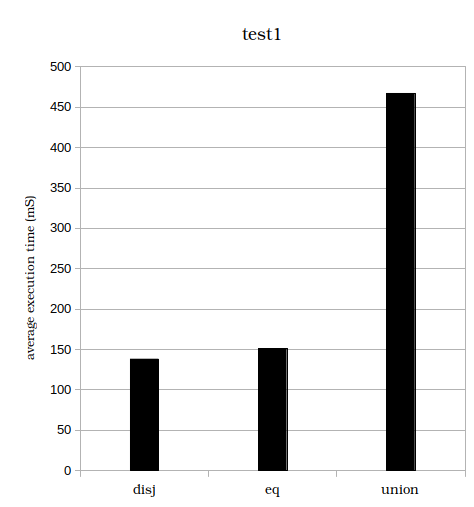
\includegraphics[scale=0.8]{images/histogram_test1.png}
\end{center}

Questa discrepanza diventa ancora più evidente aumentando le dimensioni degli insiemi, come illustrato nel prossimo paragrafo.\\

\subsubsection{test11 - insiemi completamente specificati (grandi)}
Nel test11 vengono testati i medesimi vincoli analizzati nel test1, inserendo però tra gli argomenti del test set un insieme completamente specificato di 20 elementi ground.\\
\clearpage
I risultati riportati dal file \texttt{times.txt} sono i seguenti:\\

\lstinputlisting{code/test11/times.txt}

Come evidente, i tempi sono molto simili per \texttt{disj}, più alti per \texttt{eq} e decisamente più alti per \texttt{union}, che impiega ora addirittura 10-11 secondi.\\

\begin{center}
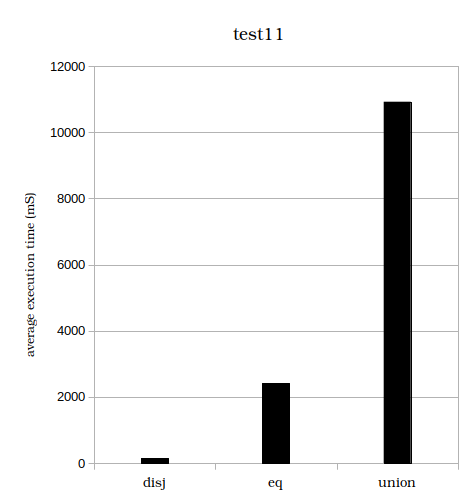
\includegraphics[scale=0.8]{images/histogram_test11.png}
\end{center}

\subsubsection{test6 - relazioni completamente specificate (piccole)}

Per quanto riguarda le relazioni, si è pensato di procedere in modo analogo a quanto fatto per gli insiemi: un'analisi dei tempi in caso di relazioni di piccole dimensioni, e un'analisi nel caso di relazioni di grandi dimensioni.

Per il primo caso, si è scelto di attivare i tempi in test6, contenente i vincoli \texttt{id}, \texttt{inv} e \texttt{comp}, con i seguenti risultati:

\lstinputlisting{code/test6/times.txt}

\begin{center}
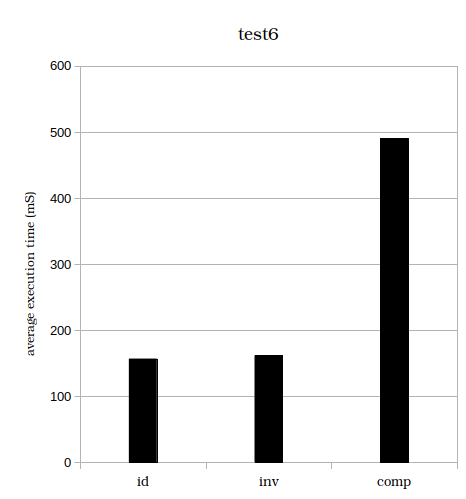
\includegraphics[scale=0.8]{images/histogram_test6.png}
\end{center}

Come previsto, anche in questo test set il collo di bottiglia è rappresentato dal vincolo più oneroso da risolvere, ossia \texttt{comp}, con risultati molto simili a quelli di \texttt{union} in test1.

\subsubsection{test12 - relazioni completamente specificate (grandi)}

Per il caso di relazioni grandi, si è scelto invece di testare i vincoli presenti in test12.\\
Per fare un confronto equo con test11, si sono scelte relazioni completamente specificate di 20 elementi ground, come appunto per test11.\\

I risultati sono i seguenti:\\ 
\lstinputlisting{code/test12/times.txt}

\begin{center}
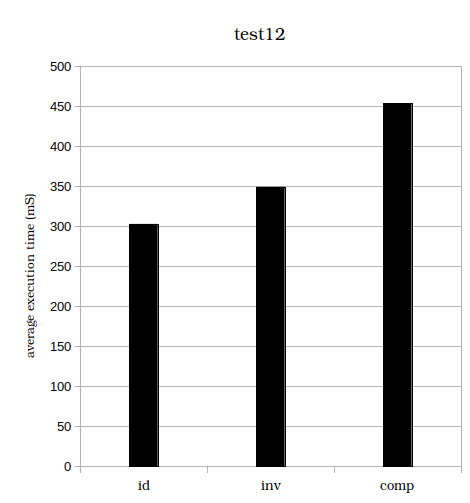
\includegraphics[scale=0.8]{images/histogram_test12.png}
\end{center}

Come si evince dai dati riportati, il vincolo \texttt{comp}, pur avendo arità 3, riesce a scalare molto meglio rispetto al vincolo \texttt{union}: i tempi restano infatti pressoché identici rispetto a quelli calcolati in test6.\\

\subsubsection{test11(bis) - insiemi parzialmente specificati (grandi)}
Come ultima analisi sui tempi d'esecuzione, si è scelto di utilizzare test11 con una lieve modifica: piuttosto che utilizzare insiemi completamente specificati di elementi ground, si è analizzato il caso di insiemi parzialmente specificati di elementi non ground, ottenuti tramite la sintassi:
\begin{verbatim} #LSetPartiallySpecifiedNotGround_20
\end{verbatim}

I risultati sono i seguenti.\\
\lstinputlisting{code/test11/times2.txt}

\begin{center}
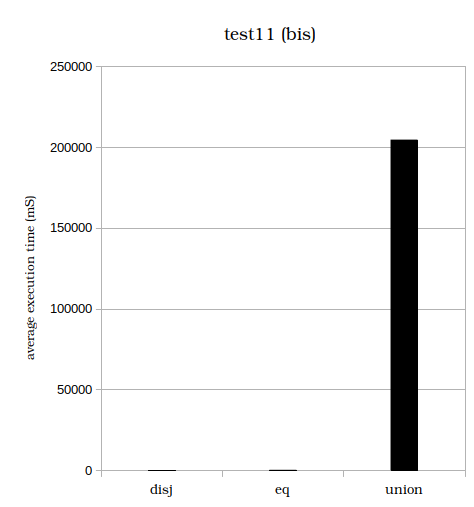
\includegraphics[scale=0.8]{images/histogram_test11bis.png}
\end{center}

Come evidente, \texttt{eq} e \texttt{disj} non risentono assolutamente di questo cambiamento.\\
Il vincolo \texttt{union} invece, impiega notevolmente di più (circa 200 secondi, più di 3 minuti).\\
Da questo dato è facile dedurre come la gestione di insiemi parzialmente specificati sia più problematica per il solver rispetto alla gestione di insiemi completamente specificati.\\

\end{document}
